{}\documentclass[letterpaper,
compress,
xcolor=x11names,
%draft,
]{beamer}
% Package imports
\usepackage{mathtools} % imports `amsmath'
\DeclareMathOperator{\sech}{sech}
\usepackage{amssymb}
\usepackage{fixltx2e}
\usepackage{lmodern}
\usepackage{movie15}
%\usepackage{media9}
\usepackage{microtype}
\usepackage{animate}
\usepackage{subcaption}
\captionsetup{compatibility=false}

% I just did this
\usepackage[english]{babel}
\usepackage[utf8]{inputenc}
\usepackage{amsmath}
\usepackage{graphicx}
\usepackage[colorinlistoftodos]{todonotes}
\usepackage{tikz}
\usetikzlibrary{tikzmark}
\usepackage{array}
\usepackage{layout}
\usepackage{multicol}
\usepackage{multirow}
\usepackage{booktabs}
%I just did this

% `beamer' configuration
\usefonttheme{professionalfonts}
\useoutertheme[subsection=false,]{miniframes}
\setbeamercolor*{alerted text}{fg=red}
\setbeamercolor*{example text}{fg=black}
\definecolor{CSU_green}{RGB}{30, 70, 43}
\definecolor{CSU_gold}{RGB}{200, 195, 114}
\setbeamercolor*{lower separation line head}{bg=CSU_gold}
\setbeamercolor*{section in head/foot}{fg=white,bg=CSU_green}
\setbeamercolor*{subsection in head/foot}{bg=white}
\setbeamercolor*{upper separation line head}{bg=CSU_gold}
\setbeamercolor*{page number in head/foot}{fg=CSU_green}
\setbeamercolor*{normal text}{fg=black,bg=white}
\setbeamercolor*{palette tertiary}{fg=black,bg=black!10}
\setbeamercolor*{palette quaternary}{fg=black,bg=black!10}
\setbeamercolor*{structure}{fg=black}
\setbeamerfont{frametitle}{shape=\scshape}
\setbeamerfont{institute}{shape=\scshape}
\setbeamerfont{section in head/foot}{shape=\scshape}
\setbeamerfont{subsection in head/foot}{shape=\scshape}
\setbeamertemplate{bibliography item}{}
\setbeamertemplate{itemize items}[ball]
\setbeamertemplate{navigation symbols}{}
\setbeamertemplate{footline}[frame number]
\usetikzlibrary{calc,arrows}
\graphicspath{{graphics/}{graphics/movies/}{graphics/images/}}
\usepackage{remreset}                  % hack to display beamer navigation
\makeatletter                          % circles even if not declaring
\@removefromreset{subsection}{section} % subsections
\makeatother                           % see: http://tex.stackexchange.com/a/2078
\setcounter{subsection}{1}             % see: https://bitbucket.org/rivanvx/beamer/issue/218

% `biblatex' configuration
\usepackage[backend=biber,
style=authortitle-comp,
]{biblatex}
\addbibresource{presentation.bib}

% `enumitem' configuration
\usepackage{enumitem}
\setlist[itemize,1]{label=\usebeamertemplate{itemize item}}
\setlist[itemize,2]{label=\usebeamertemplate{itemize subitem}}
\setlist[itemize,3]{label=\usebeamertemplate{itemize subsubitem}}
\DeclareMathOperator{\sinc}{sinc}


% `graphicx' configuration
\usepackage{graphicx}
\begin{document}
	\title{Vectors and Plotting}
	%\subtitle{MATH-151:  Mathematical Algorithms in Matlab}
	\author{MATH-151:  Mathematical Algorithms in Matlab}
	\date[202X]{September 6, 2023}
	\titlegraphic{
\includegraphics[height = 3cm]{CSU_Ram_Logo.jpg}}



%%%%%%%%%%%%%%%%%%%%%%%%%%%%%%%%%%%%%%%%%%%%%%%%%%%%%%

\begin{frame}
\titlepage
\end{frame}
%%%%%%%%%%%%%%%%%%%%%%%%%%%%%%%%%%%%%%%%%%%%%%%%%%%%%%%%%
\section{Vectors}

\begin{frame}{What is a Vector?}
	\footnotesize
	\begin{itemize}
		\item For coding, a vector is an ordered collection of values.
		\begin{center}
			Ex: \texttt{v = [1 0 -1 0 1 0 -1 0 1]}
		\end{center}
		\item This will help us keep track of a whole lot of things all at once without having to make up new variable names for each value!
		\item There are a few different ways we can think about or use vectors in code
		\begin{itemize}
			\item \underline{Data sets}: Vectors can be used to store data sets for a common variable, with the order representing which subject that sample was taken
			\begin{center}
				\texttt{height = [68 62 73 67 76]}
			\end{center}
			\item \underline{Discretization of a function}: Since a continuous function is made up of infinite values, we can use vectors to represent our functions at a number of known points
			\begin{center}
				if \texttt{x = [0 pi/2 pi 3*pi/2 2*pi]}, then \texttt{cos(x) = [1 0 -1 0 1]}
			\end{center}
			\item \underline{Physical/Mathematical sense}: We won't use this as much, but we can also represent vectors as a physical magnitude and direction, or the output/solution to a linear system
		\end{itemize}
	\end{itemize}
\end{frame}

%%%%%%%%%%%%%%%%%%%%%%%%%%%%%%%%%%%%%%%%%%%%%%%%%%%%%%%%%

\begin{frame}{Generating Special Vectors}
	\footnotesize
	\begin{itemize}
		\item Zeros and Ones: We can use the \texttt{zeros} or \texttt{ones} functions to initialize a vector or zeros or ones.
		\begin{center}
			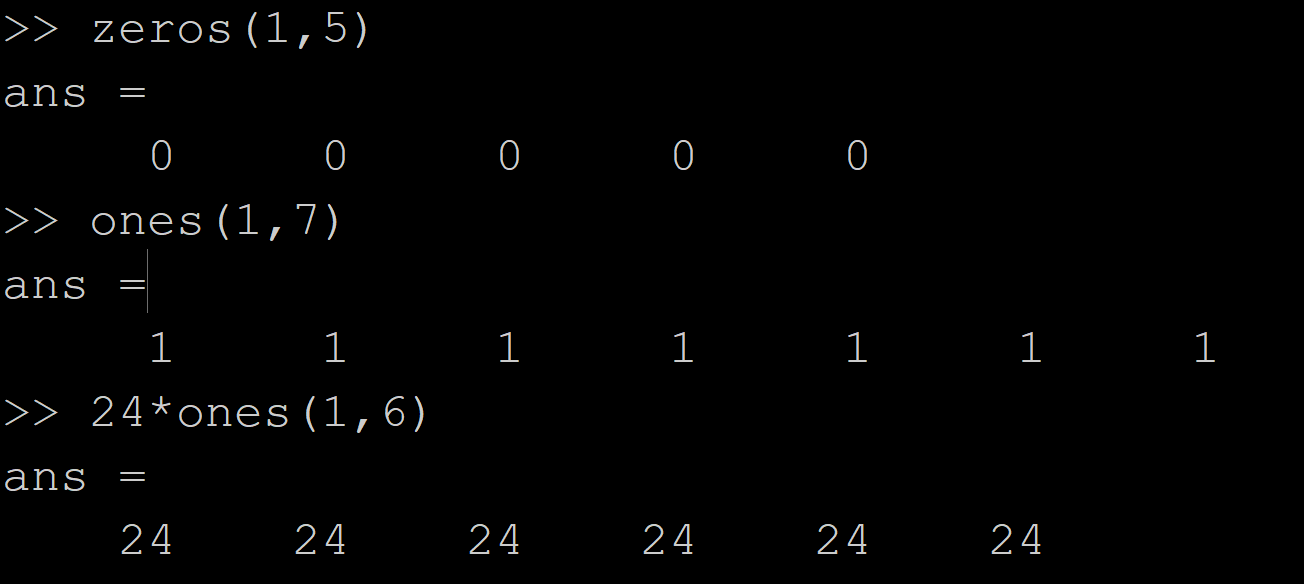
\includegraphics[height = 1.25cm]{ones_and_zeros.png}
		\end{center}
		\item Uniformly Spaced Vectors: If we have end points and a step size, we can create a vector using \texttt{start\_pt:step\_size:end\_pt}. Or if we want a number of points we can use \texttt{linspace}
		\begin{center}
			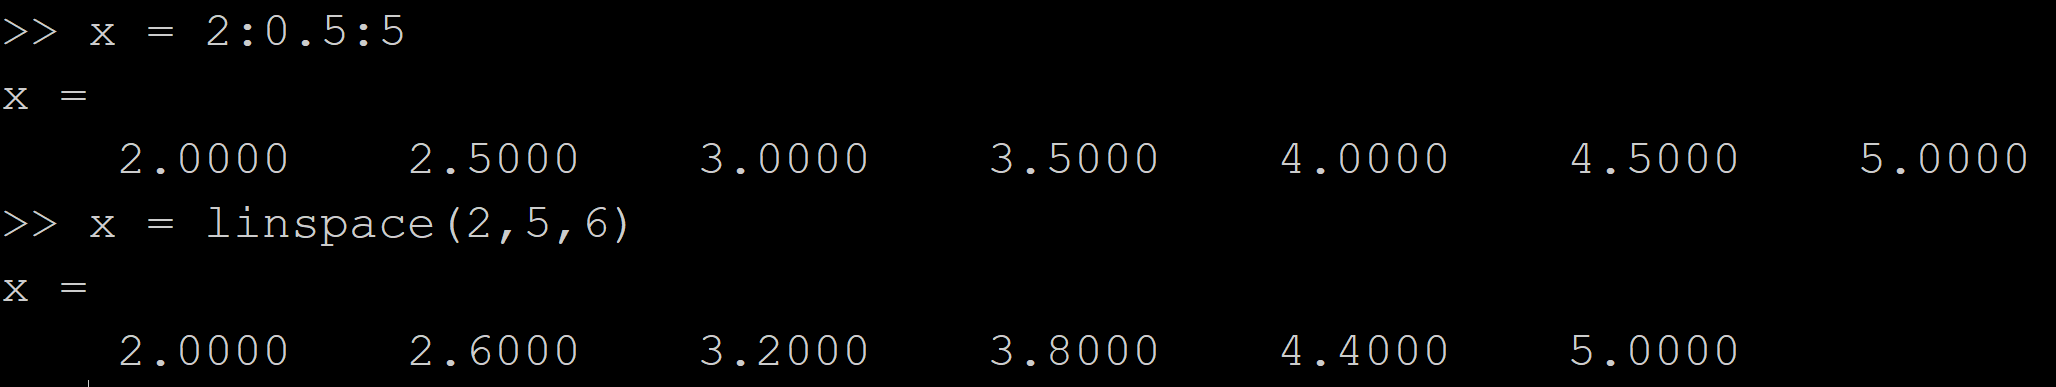
\includegraphics[height = 1.25cm]{uniform_vectors.png}
		\end{center}
		\item Random Vectors: Sometimes we want to apply random noise to a vector (happens a lot in simulation), we can generate a uniform random variable using \texttt{rand}, or normally-distributed using \texttt{randn}
		\begin{center}
			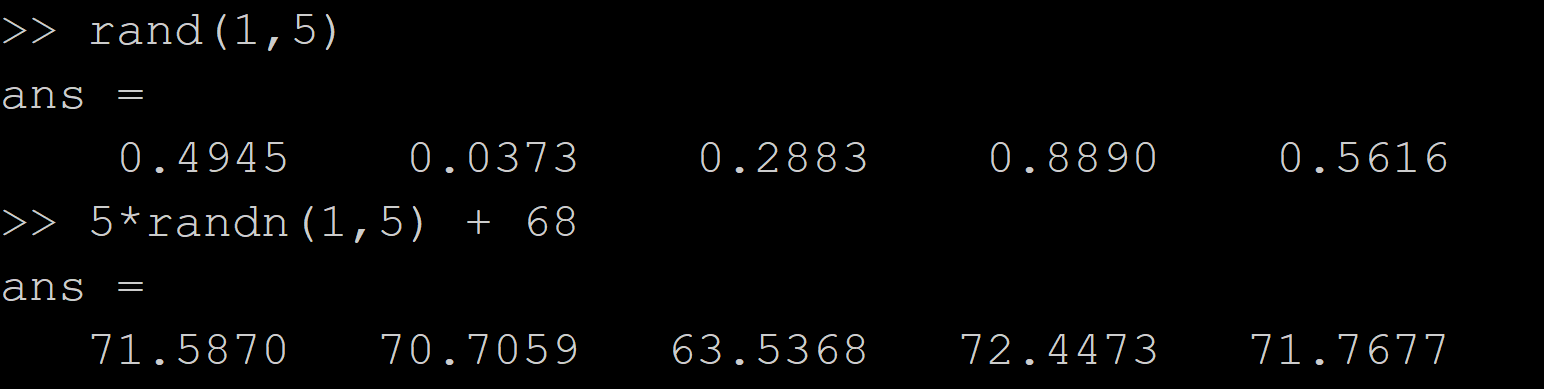
\includegraphics[height = 1.25cm]{random_vectors.png}
		\end{center}
	\end{itemize}
\end{frame}

%%%%%%%%%%%%%%%%%%%%%%%%%%%%%%%%%%%%%%%%%%%%%%%%%%%%%%%%%

\begin{frame}{Using Vectors}
	\footnotesize
	\begin{columns}
		\begin{column}{0.75\linewidth}
			\begin{itemize}
				\item Vectors are composed of \textbf{elements}, each of which has a corresponding \textbf{index} from 1 to N. We can extract a specific value by knowing its index.
				\item We can do arithmetic with either a \textbf{scalar} or element-wise with a vector of the same size.
				\begin{itemize}
					\scriptsize
					\item (Note: For multiplying two vectors we use \texttt{.*} instead of just \texttt{*}, the same for \texttt{.\^{}} when doing powers)
				\end{itemize}
				\item Many mathematical functions we know will also operate on element-wise.
				\item Another helpful tool will be that the \texttt{length} function will return the length of our vector!
			\end{itemize}
		\end{column}
		\begin{column}{0.25\linewidth}
			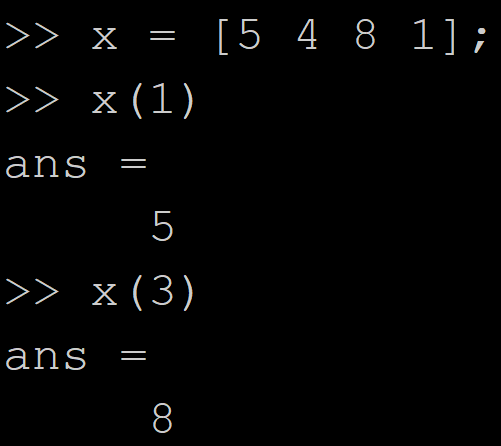
\includegraphics[width = \linewidth]{vector_elements.png}
			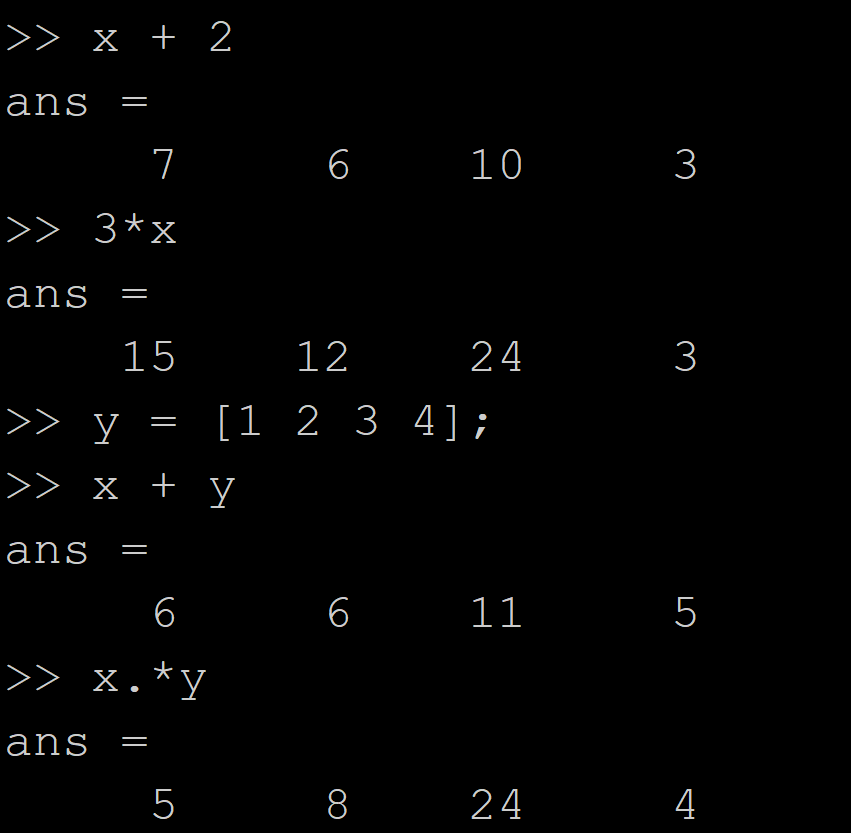
\includegraphics[width = \linewidth]{vector_arithmetic.png}
			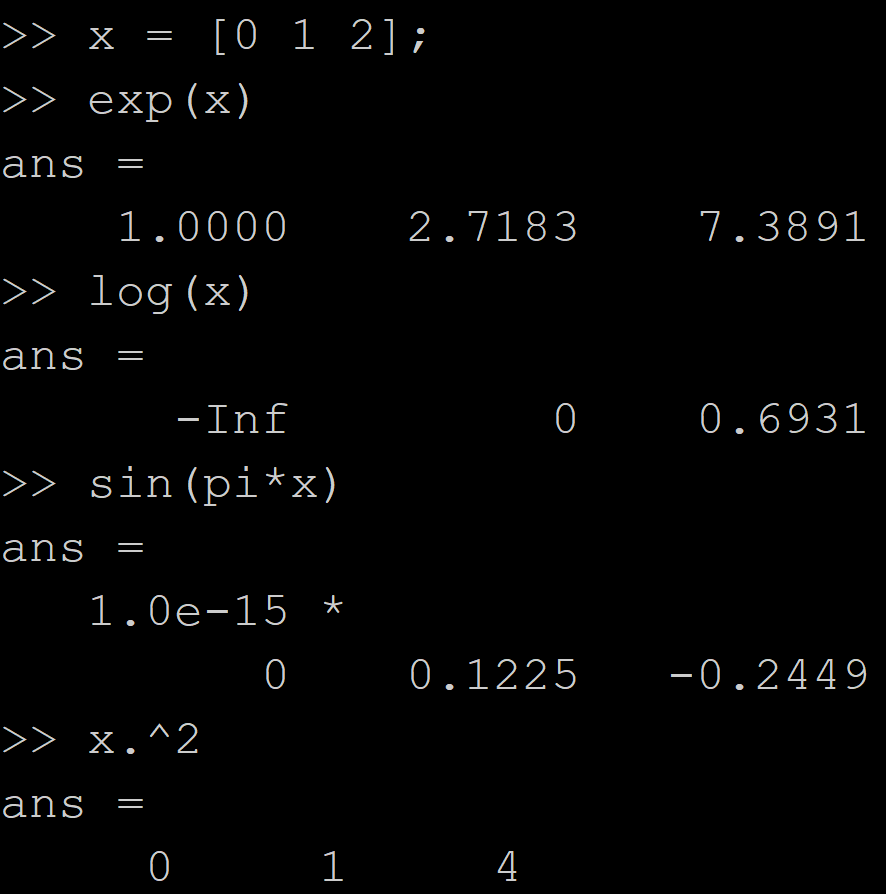
\includegraphics[width = \linewidth]{vector_functions.png}
		\end{column}
	\end{columns}
\end{frame}

%%%%%%%%%%%%%%%%%%%%%%%%%%%%%%%%%%%%%%%%%%%%%%%%%%%%%%%%%

\begin{frame}{Vector Use in Loops}
	\footnotesize
	\begin{itemize}
		\item In some cases, we want to generate a vector that depends on earlier elements of the vector
		\begin{itemize}
			\item Sequences, integration, solving differential equations
		\end{itemize}
		\item A fun example of this is the Fibonacci Sequence, we start with 1, 1, then each value is the sum of the two that come before it. This is represented mathematically as 
		\begin{equation*}
			x_n =  \begin{cases}
				1 & \text{if } n=1 \\
				1 & \text{if } n=2 \\
				x_{n-2} + x_{n-1} & \text{otherwise}
			\end{cases}
		\end{equation*}
		\item Lets see it done in Matlab
		\begin{center}
			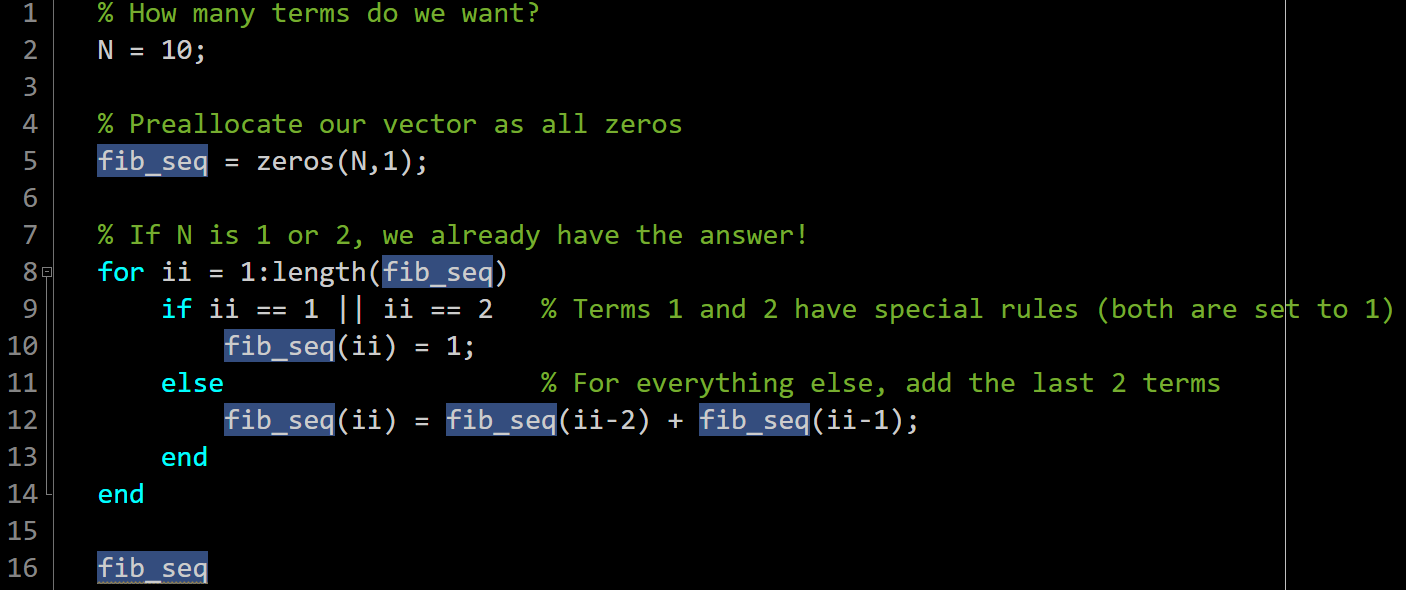
\includegraphics[height = 3cm]{fib_seq.png}
		\end{center}
	\end{itemize}
\end{frame}

%%%%%%%%%%%%%%%%%%%%%%%%%%%%%%%%%%%%%%%%%%%%%%%%%%%%%%%%%
\section{Plotting}

\begin{frame}{Plotting Vectors}
	\footnotesize
	\begin{columns}
		\begin{column}{0.6\linewidth}
			\begin{itemize}
				\item As you noticed, I didn't show the values of \texttt{fib\_seq} on the previous slide. There is a more efficient way to look at vectors, that is by plotting them! Which we can do just by \texttt{plot(fib\_seq)}	
				\begin{itemize}
					\item<2-> With a little more TLC, we can make the plot a lot easier to understand!
				\end{itemize}
				\item<3-> We can also plot functions! Let's use the plot function to see what $x^3 - 2\sin(x\pi) + 1$ looks like for $-2 < x < 2$.\\
				\begin{center}
					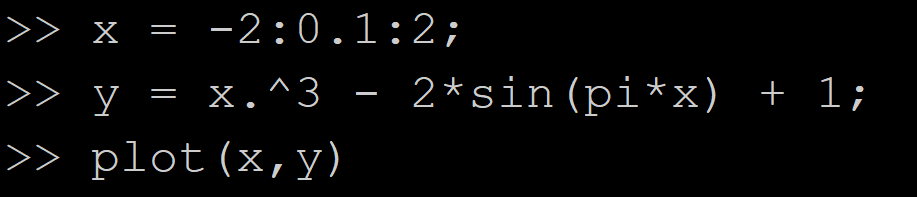
\includegraphics[width = 5cm]{function_plot_commands.png}
				\end{center}
				\item<3-> Lets use this plot to show how to make plots look better!				
			\end{itemize}
		\end{column}
		\begin{column}{0.4\linewidth}
			\only<1>{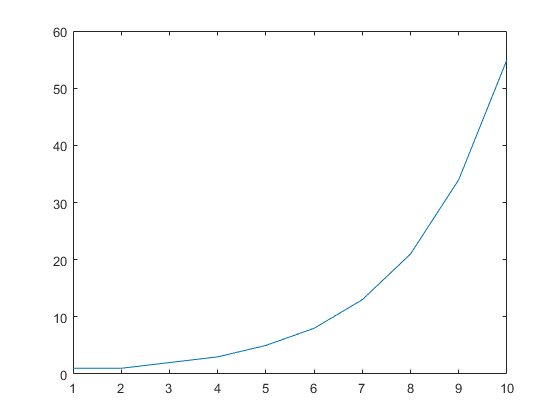
\includegraphics[width = \linewidth]{fib_seq_plot.png}}\only<2->{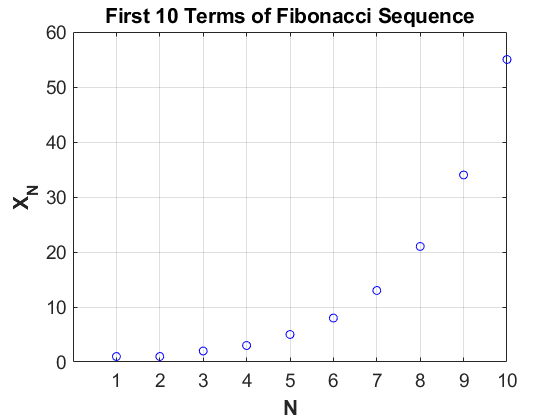
\includegraphics[width = \linewidth]{fib_seq_plot_Pretty.png}} \\
			\onslide<3->{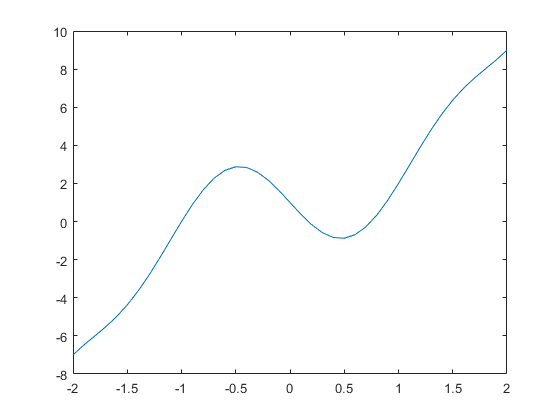
\includegraphics[width = \linewidth]{function_plot.png}}
		\end{column}
	\end{columns}
\end{frame}

%%%%%%%%%%%%%%%%%%%%%%%%%%%%%%%%%%%%%%%%%%%%%%%%%%%%%%%%%

\begin{frame}{Axis Options}
	\footnotesize
	\begin{columns}
		\begin{column}{0.6\linewidth}
			\begin{itemize}
				\item Let's look at what we can do to give this plot a makeover!
				\item<2-> First, let's change how the data is being plotted \\
				\texttt{plot(x, y, 'rx:')}
				\begin{itemize}
					\item The \texttt{r} makes the data plot in red
					\item \texttt{x} says to display an x on the vector points
					\item \texttt{:} indicates to draw a dotted line between points 
					\item Use \texttt{help plot} for more options!
				\end{itemize}
				\item<3-> Now, lets turn on a grid \\
				\texttt{grid on;}
				\item<4-> The y-axis is not centered at 0. Lets do -2 to 2 on the x-axis and -10 to 10 on the y-axis \\
				\texttt{xlim([-2 2]); ylim([-10 10]);}
			\end{itemize}
		\end{column}
		\begin{column}{0.4\linewidth}
			\only<1>{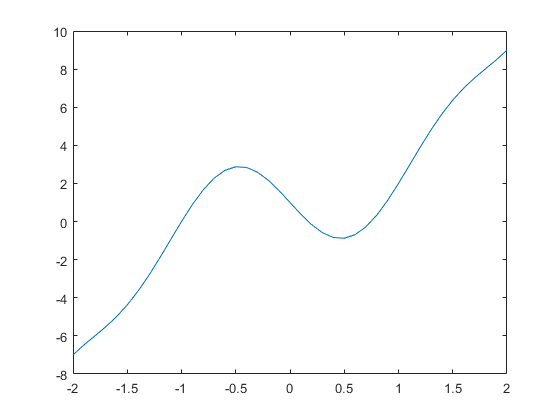
\includegraphics[width = \linewidth]{function_plot.png}}
			\only<2>{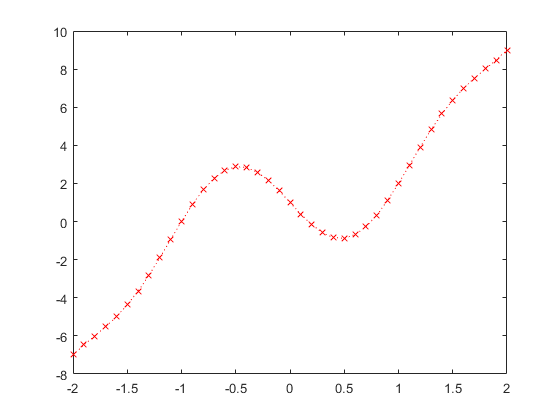
\includegraphics[width = \linewidth]{function_plot2.png}}
			\only<3>{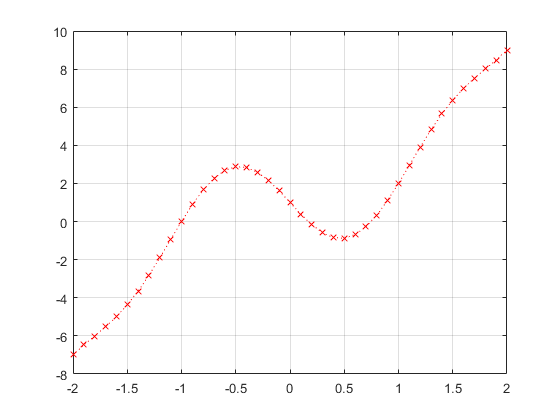
\includegraphics[width = \linewidth]{function_plot3.png}}
			\only<4>{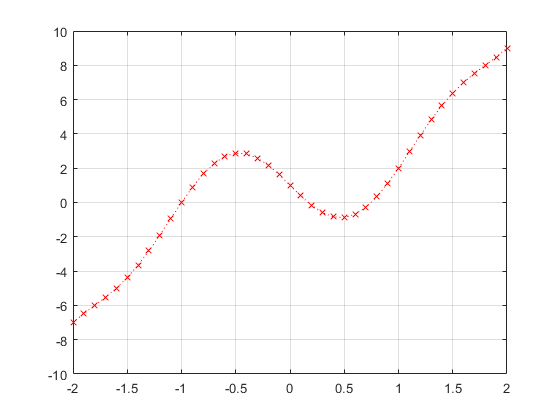
\includegraphics[width = \linewidth]{function_plot4.png}}
		\end{column}
	\end{columns}
\end{frame}

%%%%%%%%%%%%%%%%%%%%%%%%%%%%%%%%%%%%%%%%%%%%%%%%%%%%%%%%%

\begin{frame}{Plot Labeling}
	\footnotesize
	\begin{columns}
		\begin{column}{0.6\linewidth}
			\begin{itemize}
				\item This is starting to look good, but what is being plotted? We should label our plot!
				\item<2-> Suppose this is a plot of an object's position vs time! Let's label our axes appropriately\\
				\texttt{xlabel('Time (s)')};\\
				\texttt{ylabel('Position (ft)');}\\
				\begin{itemize}
					\item Note: The \texttt{' ... ' } tell Matlab that everything is a \textbf{string}, or to treat the inside as text
				\end{itemize}
				\item<3-> Finally, lets give it a title.\\
				\texttt{title('Good Lookin Plot!');}
				\item<4-> Wow! Look at that glow up!
			\end{itemize}
		\end{column}
		\begin{column}{0.4\linewidth}
			\only<1>{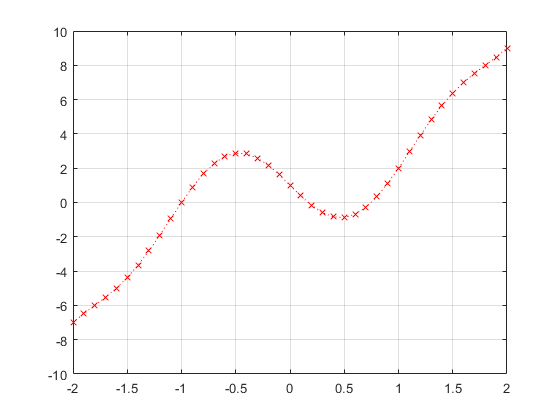
\includegraphics[width = \linewidth]{function_plot4.png}}
			\only<2>{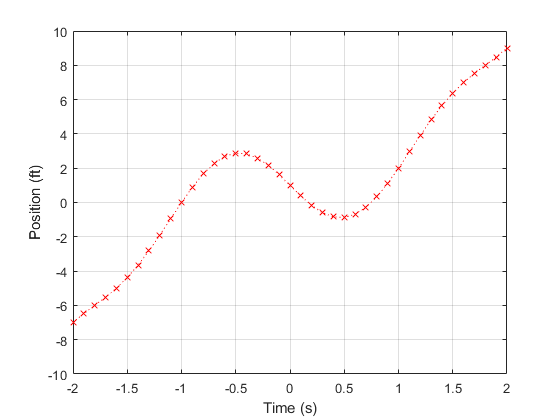
\includegraphics[width = \linewidth]{function_plot5.png}}
			\only<3>{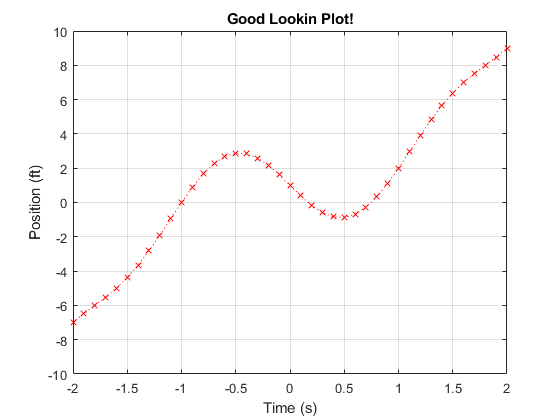
\includegraphics[width = \linewidth]{function_plot6.png}}
			\only<4>{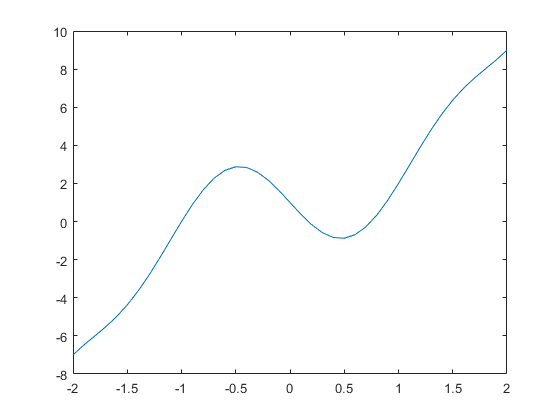
\includegraphics[width = \linewidth]{function_plot.png}}
			\only<4>{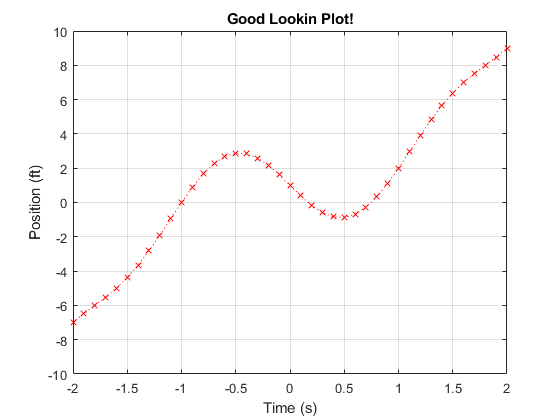
\includegraphics[width = \linewidth]{function_plot6.png}}
		\end{column}
	\end{columns}
\end{frame}

%%%%%%%%%%%%%%%%%%%%%%%%%%%%%%%%%%%%%%%%%%%%%%%%%%%%%%%%%
\begin{frame}{Multiple Plots}
	\footnotesize
	\begin{itemize}
		\item If we tried to plot something new, it would get rid of all our hard work. We don't want that! So we have two options
		\begin{itemize}
			\item If we want a new plot. We can enter \texttt{figure();} and open a new plot window.
			\item If we want to add to our existing plot we can use \texttt{hold on;} to tell Matlab to hold onto the plot as is.\\
			\texttt{hold on;} \\
			\texttt{plot(x, sin(pi*x), 'k-');}\\
			\texttt{legend('x\^{}3 - 2sin(pi*x) + 1', 'sin(pi*x)')} 
		\end{itemize}
		\item There are a lot more options you can use for making plots!
	\end{itemize}
	\begin{center}
		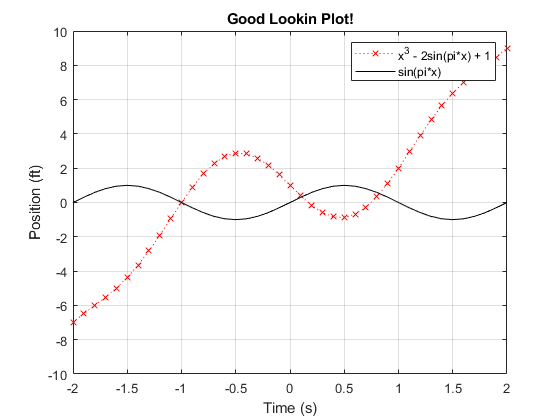
\includegraphics[height = 3.5cm]{function_plot7.png}
	\end{center}
\end{frame}

%%%%%%%%%%%%%%%%%%%%%%%%%%%%%%%%%%%%%%%%%%%%%%%%%%%%%%%%%
\end{document}